%!TEX root = main.tex

\documentclass[../main.tex]{subfiles}

\begin{document}

\chapter{Description of Slide Guitar Synthesis Model}
In this section, we introduce the synthesis model which was developed based on the theory from the Introduction. After the model has been introduced, there will be an exploration of the limitations of the design and the theoretical reasons behind them.

\section{Introduction of Architecture}
The slide guitar synthesizer developed in this thesis is heavily influenced by the model introduced in \citetwo{pakarinen_virtual_2008} and \citetwo{puputti_real-time_2010}. Modifications were made during development and they will be explained as they are introduced. Audio examples will also be provided in an effort to facilitate an aurally intuitive understanding of the model by bridging the gap between the theoretical design and the perceptual/experiential end result.

\subsection{Diagram Conventions}
The following conventions will be adhered to in this sections diagrams. This was done to improve clarity and reduce ambiguity as compared to the diagrams from the original papers \citetwo{pakarinen_virtual_2008} and \citetwo{puputti_real-time_2010}. Figure \ref{fig:slide_synth} serves an illustrative example.

In synthesis systems signals can functionally divided into two different categories: control signals and audio signals. This is illustrated by the use of dashed lines for control signals, and the use solid lines for audio signals. It is also common that the control signals are run at a sampling rate which is lower than or equal to the audio rate. This has been represented by the use of different indices for the time-index. $[m]$ represents a signal at the control-rate while $[n]$ represents a signal at the audio-rate. It is possible to have a control signal at the audio rate as is illustrated by $L[n]$ in figure \ref{fig:slide_synth}.

\subsection{Single String Slide Synthesizer}

\begin{figure}[h]
    \centering
    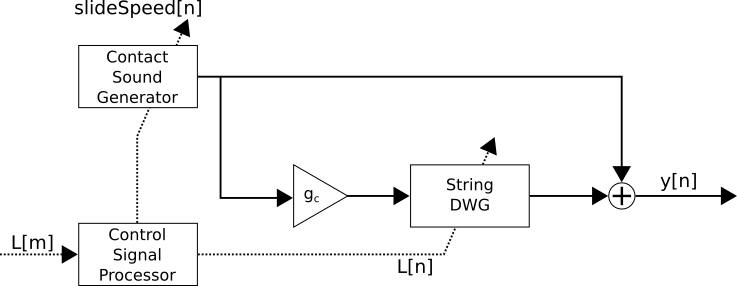
\includegraphics[scale=.65]{./images/diagrams/slideSynth.png}
    \caption{High level architecture for a single string slide synthesizer}
    \label{fig:slide_synth}
\end{figure}

The highest-level component of the synthesis system is depicted in figure \ref{fig:slide_synth}. This is a synthesizer for a single string where the pitch is controlled by a slide. Similar to the model introduced in Chapter 2, this consists of a module which represents a variable length string digital waveguide as well as a contact sound generator for the string/slide surface interactions. 

The first new addition is a gain block which controls the coupling between the longitudinal motion of the slide and the transverse vibrations of the string. The CSG model only considers with longitudinal motion in its algorithm. This phenomena was experimentally observed on a per string basis, as will be shown in Chapter 3. There is also an anti-aliasing filter added to the output, as the changing of the DWG length during synthesis can be viewed as a re-sampling operation and the appropriate measures need to be in place to prevent unwanted artifacts such as aliasing. 

The Control Signal Processor is another new block which will be more carefully detailed in the next section. It was placed here to remove the need for the individual objects to perform any processing on the control signals themselves. This improves computational efficiency by removing redundant computations as well as ensures all the constituent components are operating on control values derived from the same source.

\subsection{Control Signal Processor}

\begin{figure}[h]
    \centering
    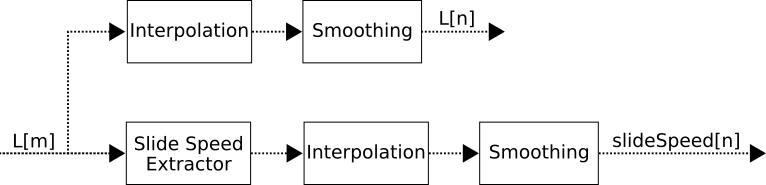
\includegraphics[scale=.65]{./images/diagrams/controlSignalProcessor.png}
    \caption{Signal flow diagram for control signal processor block}
    \label{fig:CSP}
\end{figure}

Figure \ref{fig:CSP} illustrates the internals of how the Control Signal Processor operates. Its input signal is the relative length control signal at control-rate. Its output signals are the the slide speed as well as relative length signal at audio-rate. The purpose of this block is to extract the speed signal as well as change the control-rate signals to audio-rate.

The interpolation is done via linear-interpolation and is where the control-rate signals are upsampled to the audio-rate. This allows more gradual changes to be implemented in the audio-rate objects which can help prevent unwanted artifacts like transients. Supposing that $R$ represents the ratio between the control-rate and audio-rate, then for each one control-sample, $R-1$ audio samples are calculated via the interpolation. In the case where the audio-rate is 48,000 kHz and the control-rate is 1 kHz then $R = \frac{48,000}{1,000} = 48$ and 47 samples would be calculated.

The smoothing helps eliminate any discontinuities which may be present in the interpolated signal. It is implemented via a 10-point moving window averager.

\subsubsection{Slide Speed Extractor}

\begin{figure}[h]
    \centering
    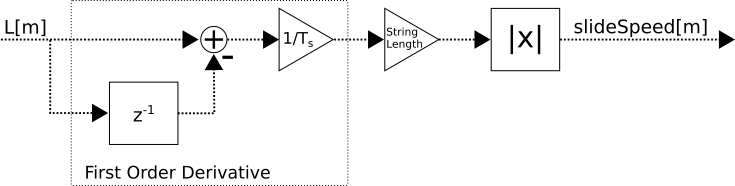
\includegraphics[scale=.5]{./images/diagrams/slideSpeedExtractor.png}
    \caption{Signal flow diagram for slide speed extractor block}
    \label{fig:SSE}
\end{figure}

Figure \ref{fig:SSE} shows a signal flow diagram for the slide speed extractor. This is extremely similar to the model introduced in \citetwo{pakarinen_virtual_2008} with some refinements for precision and clarity. Functionally it operates in the following manner. The first step is to take a difference between two consecutive samples and divide this by the sampling period. This is an approximation of the first derivative and has units of $\frac{\Delta \text{relative length}}{\text{sec}}$. The next step is to convert this from a relative length to an absolute length through multiplication by the length of a string in meters. This produces the absolute slide velocity in $\frac{\text{meters}}{\text{sec}}$. From there, the absolute value is taken to convert the velocity to a speed as the Contact Sound Generator is agnostic to the direction the slide moves.

\subsection{String DWG}

\begin{figure}[h]
    \centering
    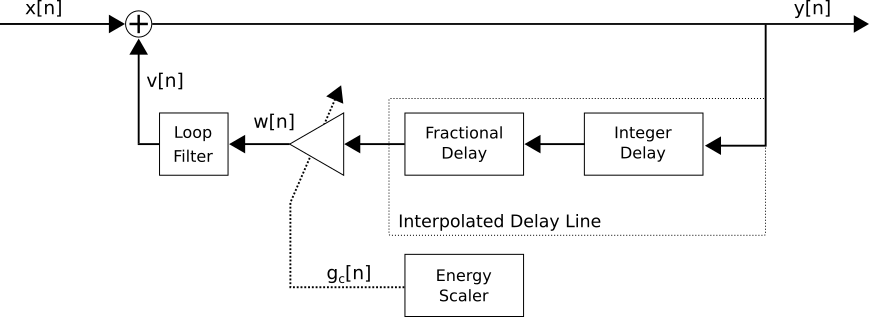
\includegraphics[scale=.5]{./images/diagrams/stringDWG.png}
    \caption{Signal flow diagram for string DWG. $L[n]$ is not depicted as every object consumes it in some fashion.}
    \label{fig:stringDWG}
\end{figure}

Figure \ref{fig:stringDWG} illustrates the string digital wave guide model. The model itself does not differ from the original as described in \citetwo{pakarinen_virtual_2008}. However, the diagram here differs in an attempt to improve clarity as compared to what was original introduced. $L[n]$ is not depicted as all the signal processing blocks rely on this in some manner. Additionally, there have been intermediate signals introduced ($v[n]$ and $w[n]$) as they were beneficial in developing the implementation code.

\subsubsection{Energy Scaler}
Figure \ref{fig:energyScaler} illustrates the signal flow diagram of the energy scaler. It implements the energy scaling as described in the Introduction chapter. The $DWGLength[n]$ signal is derived from the $L[n]$ signal via the equation $Pitch_{F_0}[n] / F_s$ where $ Pitch_{F_0}[n] = \frac{OpenString_{F_0}}{L[n]}$ and $OpenString_{F_0}$ is the fundamental frequency of the string when $L[n] = 1$.

\begin{figure}[h]
    \centering
    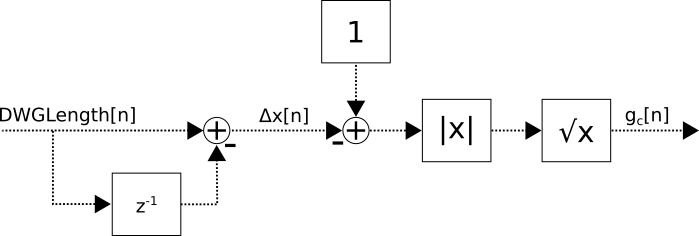
\includegraphics[scale=.5]{./images/diagrams/energyScaler.png}
    \caption{Signal flow diagram for energy scaler block}
    \label{fig:energyScaler}
\end{figure}

\subsubsection{Loop Filter}
The loop filter is implemented via a single-pole design with the following transfer-function:

\begin{equation}
    H(z) = g \frac{1 + a}{1 + a z^{-1}}
    \label{eqn:one-pole}
\end{equation}
where $a$ controls the cut-off frequency and $g$ controls the gain. The $a$ and $g$ parameters are interpolated via a first-order polynomial as described in \citetwo{valimaki_development_1998} using the values specified in tables 1 and 2 of the same paper.

\subsection{Contact Sound Generator}
Two varieties of the Contact Sound Generator exist, corresponding to the two different varieties of strings which which exist. First, the unwound approach will described which models the sound produced when the slide interacts with the smooth surface of an unwound string. After this, the more complex wound string variant will be examined in detail.

\subsubsection{Unwound Strings}
Figure \ref{fig:CSG_unwound} shows the signal flow diagram for the unwound Contact Sound Generator. The unwound strings have a substantially simpler algorithm as the sound is generated from two smooth surfaces interacting with each other. It is more akin to a friction sound generator as opposed to an impact sound, which matches the interaction between the surfaces. This contact noise can easily be modeled by low-pass filtered white noise which has its amplitude scaled by the slide's speed. A user-tunable parameter for the overall contact sound level is placed at the end of the chain. This does not different from the original design described in \citetwo{pakarinen_virtual_2008} and implemented in \citetwo{puputti_real-time_2010}.

\begin{figure}[h]
    \centering
    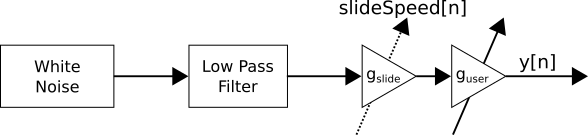
\includegraphics[scale=.5]{./images/diagrams/CSG_unwound.png}
    \caption{Signal flow diagram for unwound CSG block}
    \label{fig:CSG_unwound}
\end{figure}

\subsubsection{Wound Strings}
Figure \ref{fig:CSG_wound} illustrates the signal flow diagram for the wound string Contact Sound Generator. The core functionality does not differ from the module which was suggested in \citetwo{pakarinen_virtual_2008} in that it uses the speed of the slide to generate a sound containing a time-varying harmonic component ($v_2[n]$) and a static component due to the longitudinal modes ($v_1[n]$). It does, however,  differ substantially from the implementation in \citetwo{puputti_real-time_2010}. Additionally, variations of different components have been implemented to experiment with different timbres as indicated by the more general ``Noise Pulse/Burst Source" and ``Harmonic Accentuator" blocks.

The longitudinal mode filter remains a 4th-order IIR using the same coefficients as specified in the original paper \citetwo{pakarinen_virtual_2008}. There is also the linked pair of gain blocks which allows the balance between the static and harmonic components to be varied. The last gain block allows the overall sound level to be specified, same as in the unwound implementation.

The first step in the wound Contact Sound Generator is to convert the incoming $slideSpeed[n]$ to a frequency based on the linear density of string windings associated with the string. This $f_c[n]$ represents the rate at which the slide/winding collisions occur. The $n_w$ parameter is stored here to keep all the information specific to the string's physical properties in a single location.

\begin{figure}[h]
    \centering
    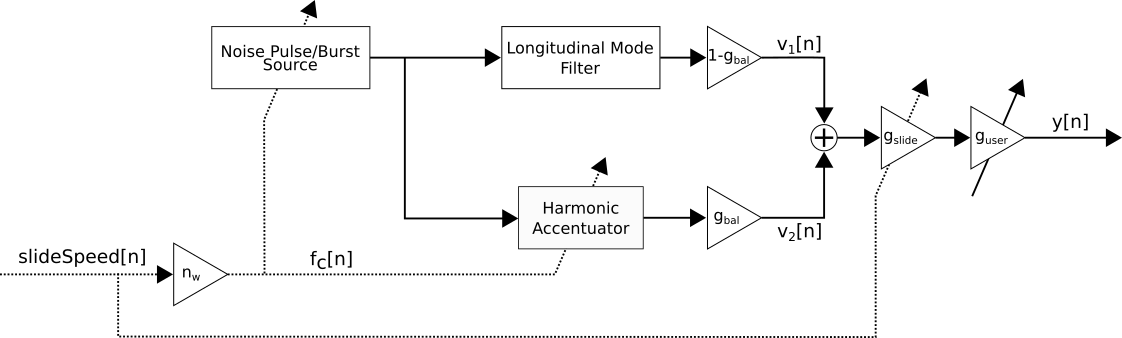
\includegraphics[scale=.5]{./images/diagrams/CSG_wound.png}
    \caption{Signal flow diagram for wound CSG block}
    \label{fig:CSG_wound}
\end{figure}

\paragraph{Noise Source}
Two variations for noise sources were developed through the course of this thesis. The first is conceptually not different from what was described in \citetwo{pakarinen_virtual_2008}, however in implementation it differs quite a bit from the version in \citetwo{puputti_real-time_2010}. The second is more akin to what was introduced in  the guqin model in \citetwo{penttinen_model-based_2006}.

\subparagraph{Noise Pulse Train}
Figure \ref{fig:NoisePulseTrain} illustrates the first variation on a noise source. It consists of absolute valued white noise which has an amplitude envelope applied to it. This amplitude envelope is generated by an impulse train which is fed into a one-pole filter. The firing rate of the impulse train is controlled by the $f_c[n]$ signal which mimics the generation of impulses from the slide hitting windings as it moves. The decay rate of the impulse response of the one-pole filter is controlled by the $T_{60}$ value measured for each string (which will be elaborated upon in the Physical Measurements chapter). The use of a one-pole filter allows the generated impulses to stack on top of each other and also benefits from being extremely computationally efficient. A DC blocker was added to help prevent unwanted DC components from tarnishing the sound as well as building up in the string digital wave guide. The difference between this an not using an absolute value block will be explained in the Sound Design chapter.

\begin{figure}[h]
    \centering
    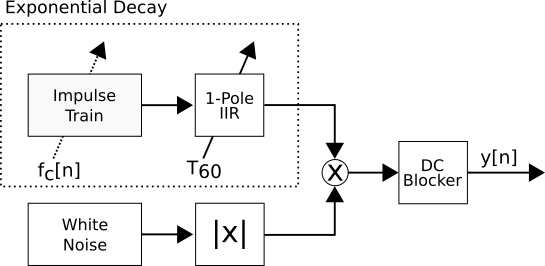
\includegraphics[scale=.5]{./images/diagrams/NoisePulseTrain.png}
    \caption{Signal flow diagram for the Noise Pulse Train generator}
    \label{fig:NoisePulseTrain}
\end{figure}

\subparagraph{Noise Burst Generator}
Figure \ref{fig:NoiseBurstGen} illustrates the second variation of a noise source. This attempts to combine the method show in \citetwo{penttinen_model-based_2006} with more string specific characteristics as shown in \citetwo{pakarinen_virtual_2008}. White noise is multiplied by an amplitude envelope as before. However, in this variation the output of the one-pole filter is hard-clipped to a value of 1. In areas of a slow slide movement the output is similar to the noise pulse train, however as the slide speed increases and more windings are struck, the signal becomes pure white noise and the harmonic component is lost. The one-pole also ensures that the starting and stopping of the noise will be more ``natural" with the addition of the decay rate. Otherwise, it would be a pure step-function and and not allow more gradual changes.

\begin{figure}[h]
    \centering
    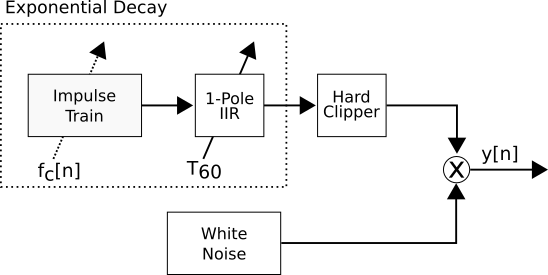
\includegraphics[scale=.5]{./images/diagrams/NoiseBurstGen.png}
    \caption{Signal flow diagram for the Noise Burst Generator}
    \label{fig:NoiseBurstGen}
\end{figure}

\paragraph{Harmonic Accentuation}
Two variations for accentuating and generating the harmonics of the wound contact sounds were investigated. The first method is the same as what is described in \citetwo{pakarinen_virtual_2008}, while the second is more akin to the method proposed for the guquin model \citetwo{penttinen_model-based_2006}.

\subparagraph{Resonator + Tanh}
The first method is a second-order resonator in series with a hyperbolic tangent function as illustrated in figure \ref{fig:ResoTanh}. The second-order resonator has its center frequency controlled by $f_c[n]$ and its $r = .99$. This configuration allows the filter to isolate the fundamental of the input signal. Assuming the input signal has a fundamental, the $\tanh$ function will introduce harmonics. The number of harmonics is controlled by the scaling factor $g$ ahead of it in the signal chain. This provides an extremely computationally efficient approach to generating the harmonics, at the expense of more fine-tuned control over the number and strength of each individual harmonic.

\begin{figure}[h]
    \centering
    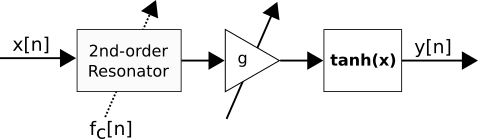
\includegraphics[scale=.5]{./images/diagrams/ResoTanh.png}
    \caption{Signal flow diagram for the Resonator + Tanh waveshaper}
    \label{fig:ResoTanh}
\end{figure}

\subparagraph{Harmonic Resonator Bank}
The second approach is illustrated in figure \ref{fig:HRB}. This method is more computationally expensive, but provides much more control over the strength, number and location of the different harmonics. It consists of a set of parallel second-order resonators whose centre frequencies are all harmonically linked to each other. At the output of each resonator is a tuneable gain coefficient to control the strength of the isolated harmonic. Six harmonics were chosen based the spectrograms in \citetwo{pakarinen_virtual_2008}.

\begin{figure}[h]
    \centering
    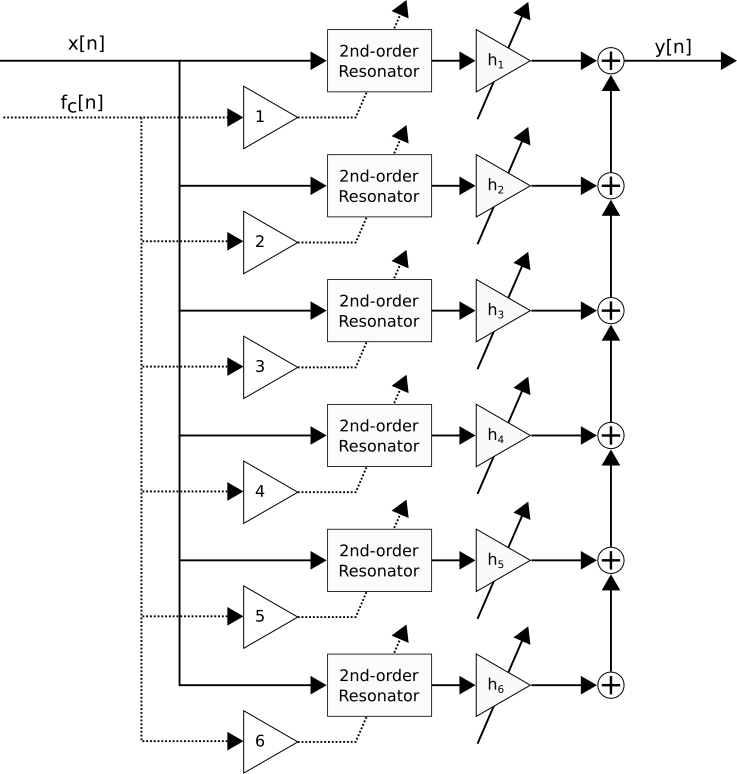
\includegraphics[scale=.5]{./images/diagrams/HarmonicResonatorBank.png}
    \caption{Signal flow diagram for the Harmonic Resonator Bank}
    \label{fig:HRB}
\end{figure}

\clearpage

\subsection{Generating Control Signals}
TODO: FILL IN HOW CONTROL SIGNALS ARE GENREATED

\section{Limitations of Model}
\subsection{Loop Filter Magnitude Response}
As detailed in \citetwo{valimaki_development_1998}, the $a$ and $g$ coefficients for this filter were derived from recordings of a professional guitar player playing several notes on all the frets of a guitar for each string. Unfortunately there is no mention of numerically how many frets were on the the guitar used in the recordings. Furthermore, there is no standardization of fret-numbers agreed upon by guitar manufacturers. Common values range are 19, 21, 22 and 24 depending on the make and manufacturer. Without a clear number of frets from which the measurements were made, it is hard to establish what range of values the relative length signal could take. This creates there situation, where physically valid fretting options create an unstable system in terms of the loop filter in certain situations. This is further complicated by the fact that slides are often used to play notes above the range of the end of the fingerboard.

Figures \ref{fig:Str1LoopMag} and \ref{fig:Str4LoopMag} illustrate this scenario more clearly. In both these figures, the magnitude response for the relative length setting of .25 (which corresponds to the 24th fret) goes above 0 dB at certain frequencies. This creates a positive feedback loop where the total amount of energy in the system increases with each iteration making the system unstable. If the relative length is maintained here for too long the output will grow unbounded and explode.

\begin{figure}[h]
    \centering
    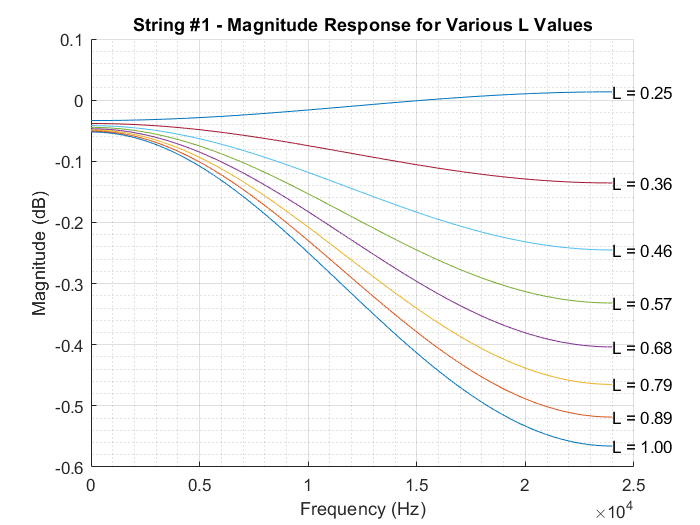
\includegraphics[scale=.65]{./images/plots/String 1 - Loop Filter Magnitude Response.png}
    \caption{Unstable Loop Filter magnitude response for high E string}
    \label{fig:Str1LoopMag}
\end{figure}

\begin{figure}[h]
    \centering
    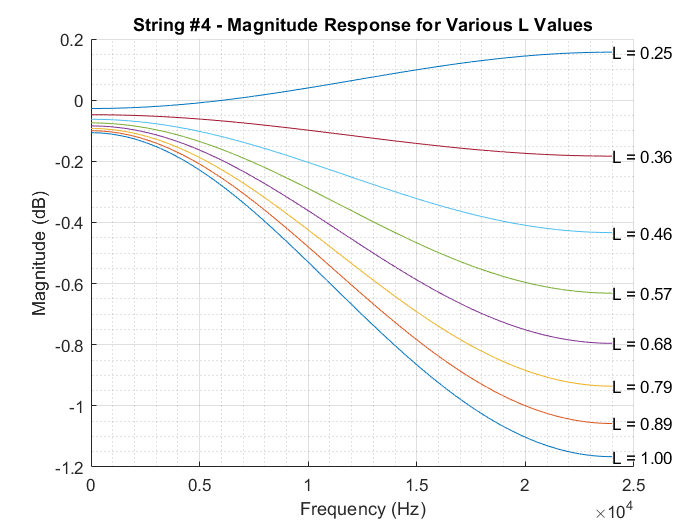
\includegraphics[scale=.65]{./images/plots/String 4 - Loop Filter Magnitude Response.png}
    \caption{Unstable Loop Filter magnitude response for D string}
    \label{fig:Str4LoopMag}
\end{figure}

Through experimentation it was determined that in order to guarantee that $|H_{loop}(\omega)| < 1$, the maximum fret value needs to be set to 21. This corresponds to $L \approx .30$. However, as shown in figure \ref{fig:Str4LoopMagStable} this results in in a frequency response where the lower frequencies are attenuated more rapidly than the higher frequencies. While stable, this is in contradiction to how the modes of a vibrating string are expected to decay. Even taking into account the various other losses (air damping, internal frictional forces, etc.) which the loop filter is approximating this is still not physically consistent and in opposition to the behavior illustrated at the various other relative string lengths.

\begin{figure}[h]
    \centering
    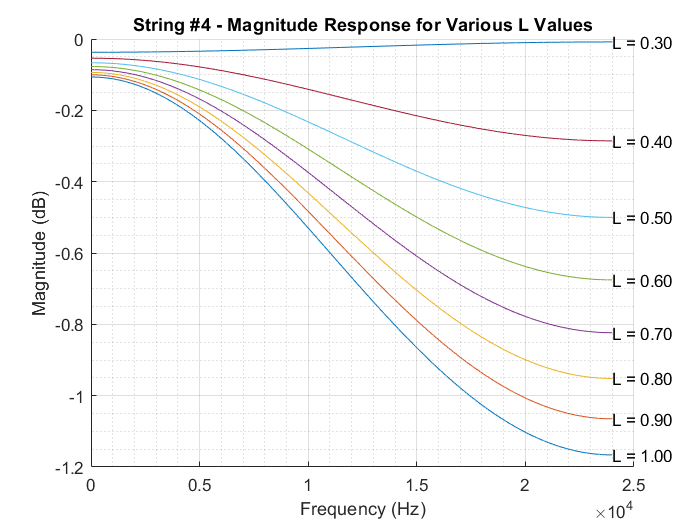
\includegraphics[scale=.65]{./images/plots/String 4 - Loop Filter Magnitude Response - stable.png}
    \caption{Stable Loop Filter magnitude response for D string}
    \label{fig:Str4LoopMagStable}
\end{figure}

Given that the filter coefficients are generated through a polynomial approximation derived from approximating the frequency response characteristics at various relative string lengths, I believe that this is an error in the process in general. It could be that the anomalous relative string lengths are not something which was captured in the original measurements. However given that the other strings do not illustrate this behavior I believe that it is more likely a limitation of the polynomial approximation used to generate the different filter coefficients. Given that the purpose of the slide is to expand the pitch palette beyond the fretboard this is a limitation when compared to the physical realities of the slide-guitar. It is often common for players to go far beyond the 24-fret and experiment with extended ranges.

In practice, to achieve this unstable state another condition needs to be imposed on the Lagrange interpolator. The total magnitude response of the loop is determined by the effects of the Lagrange interpolation filter as well as the loop filter as they are in series and the integer delay line has a unity gain. When approximating a fractional delay, the Lagrange interpolator tends to act as a low-pass filter whose attenuation at the higher-frequencies is greater than then amplification of the loop filter in an unstable state. However, if not required, then the Lagrange filter will act as a pure integer delay and have a flat magnitude response and the overall system would be unstable due to the aforementioned positive feedback. This condition occurs when the fractional component of the total digital waveguide length can be achieved via the via phase delay of the loop filter. The relative string length can be expressed as:

\begin{equation}
    L = \frac{OpenString_{F_0}}{F_s} \times DWGLength    
\end{equation}

For a given open-string fundamental frequency and sampling rate, the appropriate digital waveguide length needs to be selected. For the D-string running at 48kHz and using an approximation of .25 for the loop filter's phase delay, the following calculation produces an unstable system without going beyond the 24th fret:

\begin{equation}
    L = \frac{146.83}{48,000} \times 82.25 \approx .2516
\end{equation}

The results of this system can be heard in the example \emph{UnstableLoopFilter-scaled.wav} and are illustrated in figure \ref{fig:UnstableLoop}. This clearly shows how the upper frequencies are amplified over time as the system maintains an unstable state. The system grows quite rapidly near the end of the signal so in order to save it as a wave, it had to be scaled to prevent clipping. It is rather difficult to hear given the high contrast in the different signal levels. In a real-time system this would likely manifest as clipping so correspondingly a clipped signal was output and can be heard in the file \emph{UnstableLoopFilter-clipped.wav}.

\begin{figure}[h]
    \centering
    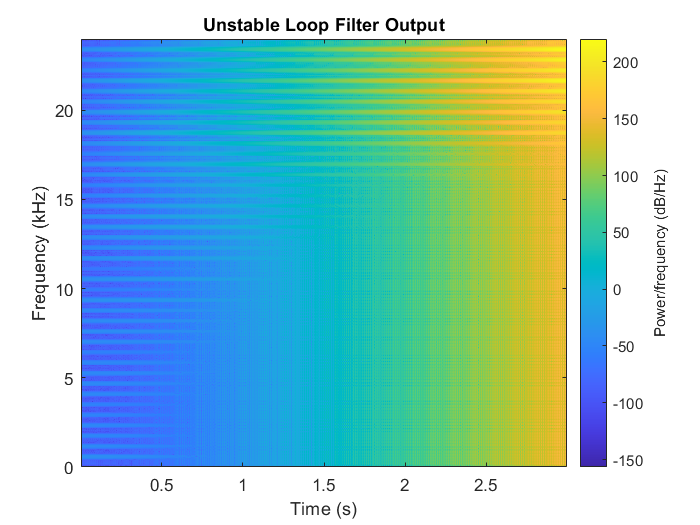
\includegraphics[scale=.65]{./images/plots/UnstableLoopFilter.png}
    \caption{Corresponds to \emph{UnstableLoopFilter-scaled.wav}}
    \label{fig:UnstableLoop}
\end{figure}

\subsection{Non-constant Phase Delay of Filters}
Both the loop filter as well as the interpolation filter illustrate non-constant phase delays. This is shown in figures \ref{fig:LagrangePhaseDelays} and \ref{fig:Str5PhaseDelays}. The loop filter illustrates this as it is an IIR filter and this is inherent in their design \citetwo{oppenheim_discrete-time_2010}. The interpolation filter is an FIR and under certain circumstances it can actually illustrate a constant delay (when the order is even and the fractional delay is .5) \citetwo{laakso_splitting_1996}. Many strings in reality exhibit some form of stiffness which results in different wavespeeds for different frequencies. This dispersion results in the observed overtones being slightly different than what an idealized string model would predict. The nature of a non-constant phase delay is similar to this, however it is more of an uncontrolled artifact here as opposed to intentional modeling. Although the values are small here, they clearly vary with the relative length signal and ultimately will affect the accuracy of the tuning from a computational standpoint. Given that this model was originally designed to be played in real-time this can easily be compensated for via ``on-the-fly" tuning by ear.

\begin{figure}[h]
    \centering
    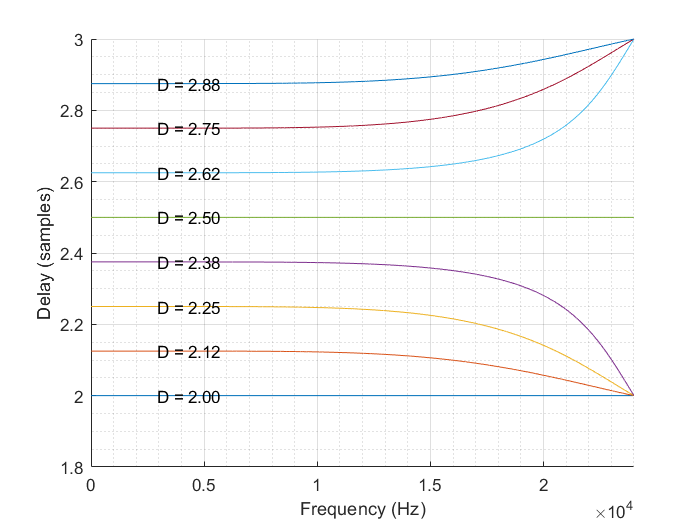
\includegraphics[scale=.65]{./images/plots/Lagrange Phase Delays.png}
    \caption{Phase delays for Lagrange interpolating filters with order = 5 at various delay values}
    \label{fig:LagrangePhaseDelays}
\end{figure}

\begin{figure}[h]
    \centering
    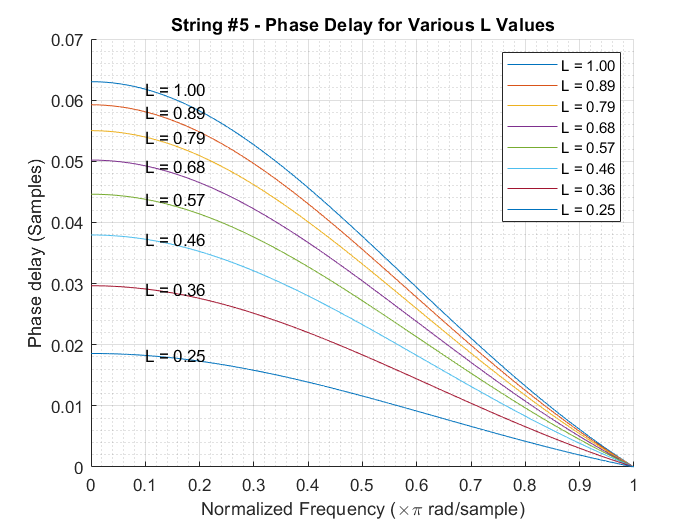
\includegraphics[scale=.65]{./images/plots/String 5 - Phase Delays.png}
    \caption{Loop Filter phase delay}
    \label{fig:Str5PhaseDelays}
\end{figure}

\subsection{Bandwidth Limitations}
One limitation, which was discovered while testing the extremes values for slide conditions, is related to bandwidth limitations inherent in a digital model. As we are simulating the system digitally here, the Nyquist rate forms the upper limit on the frequencies which can be represented. For a system run at 48 kHz, this corresponds to 24 kHz. In this particular model, there is a permanent loss in harmonics when you slide upwards as well as a limitation in the number of harmonics when sliding downwards. These are illustrated in figures \ref{fig:ExtremeDownwardSlide} and \ref{fig:ExtremeUpwardSlide} as well as the files \emph{ExtremeDownwardSlide-NoLoopFilter.wav} and \emph{ExtremeUpwardSlide-NoLoopFilter.wav}. The loop filter has been disabled in order to allow the harmonics to exist for longer and help illustrate the issue. The attenuation which occurs in these examples is due to the effects of the interpolation filter as well as the energy scaler.

\begin{figure}[h]
    \centering
    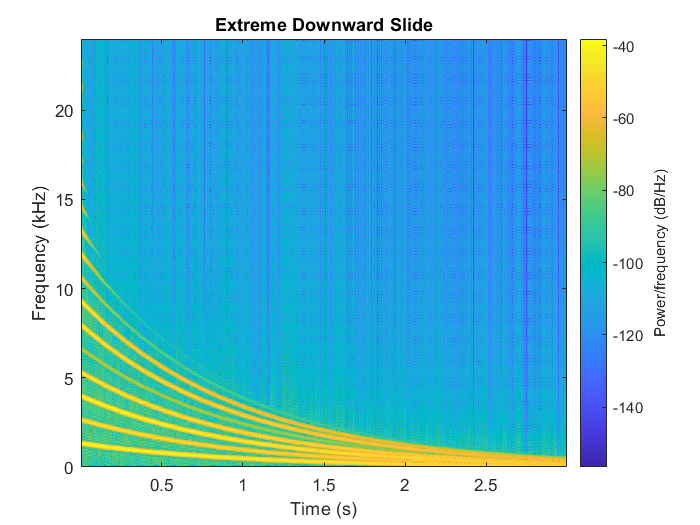
\includegraphics[scale=.65]{./images/plots/ExtremeDownwardSlide_NoLoopFilter.png}
    \caption{Extreme downward slide with the Loop Filter disabled to help illustrate reduced harmonics}
    \label{fig:ExtremeDownwardSlide}
\end{figure}

\begin{figure}[h]
    \centering
    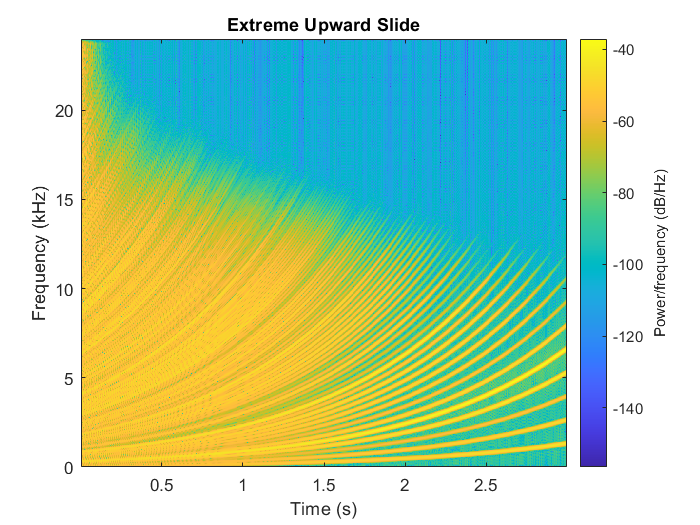
\includegraphics[scale=.65]{./images/plots/ExtremeUpwardSlide_NoLoopFilter.png}
    \caption{Extreme upward slide with Loop Filter disabled to help illustrate reduced harmonics}
    \label{fig:ExtremeUpwardSlide}
\end{figure}

In order to eliminate the effects of the interpolation filter and energy scaler, the same sweep was run on a string digital waveguide model which consists only of an integer delay line. Figures \ref{fig:StringDWGIntAsc} and \ref{fig:StringDWGIntDesc} illustrate the spectra of this scenario. These can be heard in \emph{StringDWGInt-Ascending.wav} and \emph{StringDWGInt-Descending.wav}. As is clearly shown in the ascending figure,  the harmonics get spaced out further apart as the fundamental frequency increases. The signal gets less spectrally dense over time as the number of harmonics is limited by the cap imposed by the sampling rate. The descending figure illustrates that the upper harmonics are gradually re-introduced as the delay line becomes longer and longer. From this, we can conclude that the loss of harmonics in the descending slide case is due to the attenuation effects of the loop and interpolation filters.

\begin{figure}[h]
    \centering
    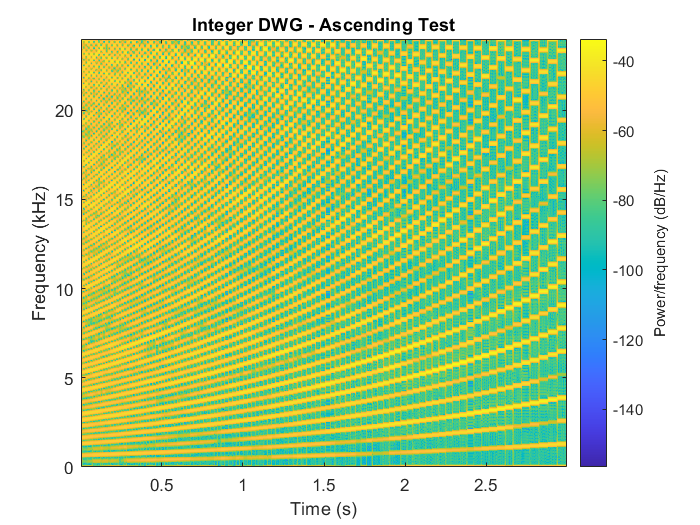
\includegraphics[scale=.65]{./images/plots/StringDWGIntAsc.png}
    \caption{Note the quantization in frequency as well as the loss of harmonics}
    \label{fig:StringDWGIntAsc}
\end{figure}

\begin{figure}[h]
    \centering
    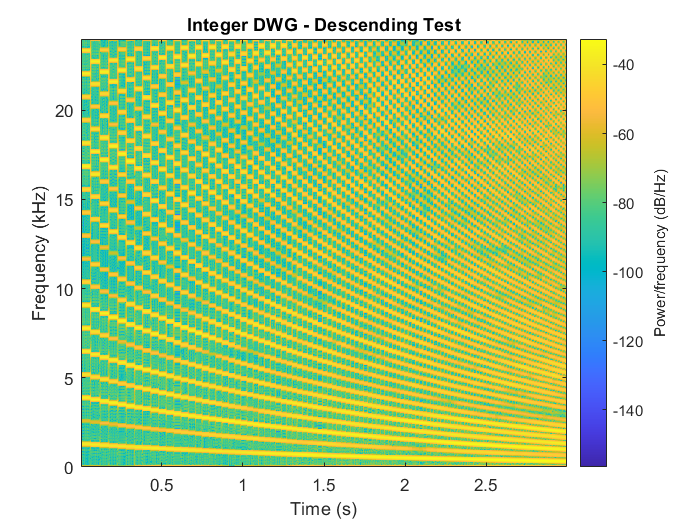
\includegraphics[scale=.65]{./images/plots/StringDWGIntDesc.png}
    \caption{Note the quantization in frequency as well as the reintroduction of harmonics}
    \label{fig:StringDWGIntDesc}
\end{figure}

It is difficult to test the physical accuracy of the complete loss of harmonics given that there is coupling between the longitudinal motion of the slide and transverse vibrations on a real-physical system (as will be shown in the chapter on physical measurements). Completely eliminating that would require a measurement setup where the moving string termination had an extremely low-coefficient of friction in relation to the string surface. The true nature of a string with a time-varying length is controversial \citetwo{pakarinen_virtual_2008}, however there is no reason why the upper harmonics of a string would be limited from a physical standpoint. The loss of the harmonics is due to the inability of the system to represent them at that sampling rate. In summary, the inherent bandwidth limitations imposed by the sampling rate create limitations on the physical accuracy of the model.

\end{document}